\documentclass[12pt,a4paper]{article}
\usepackage[margin=2.2cm]{geometry}

\usepackage{hyperref}
% \usepackage[utf8]{inputenc}
% \usepackage[T1]{fontenc}
\usepackage{float}
\usepackage{xcolor}
\usepackage{enumitem}
\usepackage{amsmath}
\usepackage{amssymb}
\usepackage{tikz}
\usetikzlibrary{arrows.meta}
\usetikzlibrary{decorations.pathreplacing}
\usepackage{amsfonts}
\usepackage{graphicx}
\usepackage{subcaption}
\usepackage{caption}
\newcommand{\dv}[2]{\frac{\mathrm{d} #1}{\mathrm{d} #2}}
\usepackage{caption}
\captionsetup[figure]{font=small} 
% \captionsetup[table]{font=small}
\usepackage[capitalize,nameinlink]{cleveref}
\usepackage{mathtools}
\newcommand{\defeq}{\vcentcolon=}
\newcommand{\eqdef}{=\vcentcolon}
\usepackage{amsmath,amssymb}
\usepackage{booktabs,tabularx,array}

% Define environments
\newtheorem{theorem}{Theorem}
\newtheorem{definition}{Definition}
\newtheorem{lemma}{Lemma}
\newtheorem{corollary}{Corollary}

% % Make all sections Plum
% \usepackage[dvipsnames]{xcolor}
% \usepackage{titlesec}
% % This automatically colors all section titles Plum
% \titleformat{\section}
%   {\color{Plum}\normalfont\Large\bfseries}{\thesection}{1em}{}
% \titleformat{\subsection}
%   {\color{Plum}\normalfont\Large\bfseries}{\thesubsection}{1em}{}
% % Shortcut for standard Orchid
% \newcommand{\spring}[1]{\textcolor{Orchid}{#1}}



% Colour Section Titles
\usepackage[dvipsnames]{xcolor}
\usepackage{titlesec}
\usepackage{enumitem}

% Current heading colour (stored as a name)
\def\currentheadingcolor{Plum}

% Section heading: Plum
\titleformat{\section}
  {\normalfont\Large\bfseries\color{Plum}}
  {\thesection}{1em}{}

% Subsection heading: Orchid
\titleformat{\subsection}
  {\normalfont\large\bfseries\color{Orchid}}
  {\thesubsection}{1em}{}

% For highlightng text
\newcommand{\skyblue}[1]{\textcolor{SkyBlue}{#1}}




\usepackage[T1]{fontenc}
\usepackage{lmodern}
\usepackage{mathtools}
\usepackage{geometry}
\usetikzlibrary{calc}
\usepackage{xcolor}
\usepackage{microtype}

\geometry{margin=27mm}
\setlength{\parindent}{0pt}
\setlength{\parskip}{0.45em}
\setlist[itemize]{topsep=3pt,itemsep=4pt,parsep=1pt}
\setlist[enumerate]{topsep=3pt,itemsep=9pt,parsep=1pt}
\hypersetup{colorlinks=true,linkcolor=black}
\newcommand{\PP}{\mathcal{P}}
\newcommand{\dd}{\mathrm{d}}
\newcommand{\qtest}{Q_{\mathrm{test}}}
\newcommand{\qtrial}{Q_{\mathrm{trial}}}
\newcommand{\rFacet}{R_{\mathrm{facet}}}
\newcommand{\rCell}{R_{\mathrm{cell}}}
\newcommand{\cones}{\mathrm{cones}}
\newcommand{\dn}{\partial_n}
\newcommand{\bubbles}{\texttt{bubbles}}
\newcommand{\midS}{\operatorname{mid}(S)}
\newcommand{\Rone}{R_{\partial T}^{1}}
\newcommand{\Rzero}{R_{\partial T}^{0}}
\newcommand{\Roneh}{R_{\partial T}^{1,h}}
\newcommand{\Rzeroh}{R_{\partial T}^{0,h}}

\title{\textbf{Notes on My Progress on Automated $C^1$ Localisation}}
\date{}
\author{}

\begin{document}
\maketitle
\vspace{-2em}

\section{Spaces}
\begin{itemize}
    \item \texttt{FB}: retain interior facet degrees of freedom (DOFs) for a Lagrange element.

    \item \texttt{el}: a broken \texttt{FB} element of degree $\dim+r$.

    \item $Q$: the function space formed using \texttt{el} over the mesh; it collects the interior facet DOFs on each cell.
\end{itemize}

Let $Q_{S_i}(T_j)$ denote the span of the interior facet basis functions associated with facet $S_i$ of cell $T_j$. Then
\begin{equation}
    Q=\bigoplus_{i,j}Q_{S_i}(T_j).
\end{equation}

\subsection{Example: triangles, ($\dim=2$, $r=1$)}

In this case, a $\text{degree}=\dim+r=3$ Lagrange element has the following DOFs.

\begin{figure}[htbp]
\centering
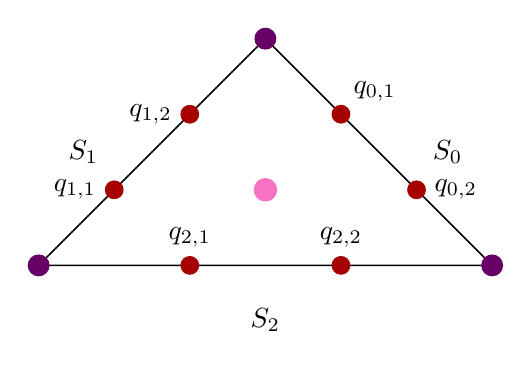
\begin{tikzpicture}[scale=0.96,
    facetnode/.style={circle,fill=red!65!black,inner sep=2.4pt},
    vertex/.style={circle,fill=violet!80!black,inner sep=2.8pt},
    interior/.style={circle,fill=magenta!55,inner sep=3pt}]
  \coordinate (v0) at (3,3.0);
  \coordinate (v1) at (0,0);
  \coordinate (v2) at (6,0);
  \coordinate (q01) at ($(v0)!1/3!(v2)$);
  \coordinate (q02) at ($(v0)!2/3!(v2)$);
  \coordinate (q12) at ($(v0)!1/3!(v1)$);
  \coordinate (q11) at ($(v0)!2/3!(v1)$);
  \coordinate (q21) at ($(v1)!1/3!(v2)$);
  \coordinate (q22) at ($(v1)!2/3!(v2)$);
  \draw[semithick] (v0)--(v1)--(v2)--cycle;
  \foreach \v in {v0,v1,v2} \node[vertex] at (\v) {};
  \foreach \v in {q01,q02,q11,q12,q21,q22} \node[facetnode] at (\v) {};
  \node[interior] at (3,1) {};
  \node[above right=1pt] at (q01) {$q_{0,1}$};
  \node[right=3pt] at (q02) {$q_{0,2}$};
  \node[left=3pt] at (q12) {$q_{1,2}$};
  \node[left=3pt] at (q11) {$q_{1,1}$};
  \node[above=3pt] at (q21) {$q_{2,1}$};
  \node[above=3pt] at (q22) {$q_{2,2}$};
  \node[right=16pt] at ($(v0)!0.5!(v2)$) {$S_0$};
  \node[left=16pt] at ($(v0)!0.5!(v1)$) {$S_1$};
  \node[below=12pt] at ($(v1)!0.5!(v2)$) {$S_2$};
\end{tikzpicture}
\caption{DOFs of a cubic Lagrange triangle.}
\end{figure}

Then, on a cell $T$,
\begin{align}
    Q(T)&=\operatorname{span}\bigl\{q_{i,j}:i=0,1,2,\ j=1,2\bigr\},\\
    Q_{S_i}(T)&=\operatorname{span}\bigl\{q_{i,j}:j=1,2\bigr\}.
\end{align}

In particular, on $S_0$, consider $q_{0,1}$ and $q_{0,2}$. These basis functions must vanish at every other DOF on the triangle. Hence they can be written as
\begin{equation}
    q_{0,1}=\lambda_1\lambda_2 p_{0,1},\qquad
    q_{0,2}=\lambda_1\lambda_2 p_{0,2},
    \qquad p_{0,1},p_{0,2}\in\PP_1(T).
\end{equation}

For $v\in Q(T)$, we have
\begin{align}
    v|_T={}&a_1q_{0,1}+a_2q_{0,2}+b_1q_{1,1}+b_2q_{1,2}
    +c_1q_{2,1}+c_2q_{2,2}.
\end{align}
Using the barycentric representations of the basis functions,
\begin{equation}
    v|_T=\lambda_1\lambda_2 p_0
          +\lambda_0\lambda_2 p_1
          +\lambda_0\lambda_1 p_2,
    \qquad p_i\in\PP_1(T).
\end{equation}

On $S_0=\{\lambda_0=0\}$, therefore,
\begin{equation}
    v|_{S_0}=\lambda_1\lambda_2\,p_0|_{S_0}.
\end{equation}
In this way,
\begin{equation}
    Q(T)|_{S_0}=\lambda_1\lambda_2\,\PP_1(S_0).
\end{equation}

\newpage

\section{Rognes and Logg Localisation}

The big idea is to isolate the cell residual by choosing a test function that annihilates every facet contribution (bubble function). Then, for each facet, we choose test functions that annihilate every other facet contribution (cones). This creates a sequence of local problems. 


\subsection{Local Cell Problems: Theory}
We assume a residual of the form
\begin{equation}
    r_T(v)=(R_T,v)_T+(R_{\partial T},v)_{\partial T}
    \qquad\text{for all }v.
\end{equation}
For the local cell problem, we consider the cell bubble function
\begin{equation}
    b_T=\prod_{i=1}^{d+1}\lambda_{x_i}^{T},
    \qquad b_T|_{\partial T}=0.
\end{equation}
Using this bubble function, we test the residual against $v=b_T\phi_i$, where $\{\phi_i\}_{i=1}^m$ is a basis for $\PP^r(T).$ In doing so, we solve
\begin{equation}
    (R_T,b_T\phi_i)_T=r_T(b_T\phi_i),
    \qquad i=1,\ldots,m.
\end{equation}
for $R_T^h \in \PP^r(T).$

\subsection{Local Cell Problems: Pablo's implementation}
\begin{enumerate}[label=\roman*)]
    \item Set $B$ to be a bubble space of degree $\dim+1$.
    This retains the interior Lagrange DOF on each element. The degree is $\dim+1$ because the bubble is one degree higher than the simplex dimension. For example, on a triangle ($\dim=2$), the bubble is cubic:
    \begin{equation}
        b_T = \lambda_1\lambda_2\lambda_3.
    \end{equation}
    % This gives the barycentric product, since an interior basis function must vanish along each edge.

    \item Define
    \begin{equation}
        \texttt{bubbles = Function(B).assign(1)}.
    \end{equation}
    Thus \texttt{bubbles} is a bubble function with its DOF set to $1$ (normalisation).

    \item Let \texttt{DG} be the discontinuous Galerkin space of degree $r$ for the $r$-degree $R_T$.

    \item Solve
    \begin{equation}
        \texttt{inner(uc, bubbles*v)*dx}
        =\texttt{residual(F, bubbles*v)*dx},
    \end{equation}
    where $\texttt{uc}$ is the $\texttt{DG}_r$ trial function, $\texttt{F}$ is the residual, and $\texttt{v}$ is the $\texttt{DG}_r$ test function.
\end{enumerate}

\subsection{Local Facet Problem: Theory}
For each facet $S$, define the cone function $\beta_S^T$ by
\begin{equation}
    \beta_S^T=\prod_{i\in I_S^T}\lambda_{x_i}^{T},
\end{equation}
where $I_S^T$ is a suitable index set such that $\beta_S^T|_F=0$ whenever $F\ne S$ is another facet of $T$.

For example, take a triangle $T$ with $S=\{\lambda_0=0\}$, so that $S$ joins vertices $v_1$ and $v_2$. Then $I_S^T=\{1,2\}$ and
\begin{equation}
    \beta_S^T=\lambda_1\lambda_2.
\end{equation}
This is a polynomial on all of $T$, not just on $S$. Its key properties are
\begin{align}
    \beta_S^T|_{\{\lambda_1=0\}\,\cup\,\{\lambda_2=0\}}&=0,\\
    \beta_S^T|_S&=\lambda_1\lambda_2.
\end{align}
Therefore the facet contributions other than $S$ vanish when testing against $\beta_S^T$.

In particular, suppose that $R_{\partial T}|_S\in\PP^r(S)$, and test with
\begin{equation}
    v=\beta_S^T\phi_i,
\end{equation}
where $\phi_i$ is a basis function of $\PP^r(S)$. The local problem for the facet $S$ is
\begin{equation}
    \bigl(R_{\partial T}|_S,\beta_S^T\phi_i\bigr)_S
    =r_T(\beta_S^T\phi_i)
     -(R_T,\beta_S^T\phi_i)_T,
    \qquad i\in I_S^T.
\end{equation}
% Transcription note: the handwritten notes use i \in I_S^T in this
% last equation, though I_S^T was previously used as the vertex index set.

\subsection{Local Cell Problem: Pablo's Implementation}
\begin{enumerate}[label=\roman*)]
    \item Define $Q$ to be the \texttt{FB} function space of broken elements of degree $\dim+q$.

    \item Define \texttt{FB} to be an \texttt{FB} space of degree $\dim$, and set
    \begin{equation}
        \texttt{cones = Function(FB).assign(1)}.
    \end{equation}
    On a triangle $T$ this gives
    \begin{equation}
        \cones|_T=C(\lambda_0\lambda_1+\lambda_1\lambda_2+\lambda_0\lambda_2),
    \end{equation}
    where $C$ is a normalisation constant. On $S=\{\lambda_0=0\}$,
    \begin{equation}
        \cones|_S=C\lambda_1\lambda_2.
    \end{equation}

    \item The right-hand side of the local problem is
    \begin{equation}
        L_f=\texttt{residual(F, Qtest)}
              -\texttt{inner(Rcell, Qtest)*dx},
    \end{equation}
    where $\qtest$ is a test function in $Q$ and $\rCell$ is the previously computed $R_T$.

    \medskip
    \textbf{\skyblue{QUESTION. How does $\qtest$ compare to the $\beta_S^T\phi_i$ used by Rognes and Logg?}}
    \medskip

    \item The left-hand side is
    \begin{equation}
    \begin{aligned}
        a_f=\texttt{both(}&\texttt{inner(Qtrial/cones, Qtest)*dS}\\
                         &\texttt{+ inner(Qtrial/cones, Qtest)*ds}\texttt{)},
    \end{aligned}
    \end{equation}
    where $\qtrial$ is a trial function in $Q$ and \texttt{both} adds the contributions from both cells sharing $S$.

    \item Let's dive deeper into the left-hand side. 
    As discussed,
    \begin{equation}
        Q=\bigoplus_{i,j}Q_{S_i}(T_j).
    \end{equation}
    On a given facet $S$, the basis functions of $Q$ can be written as
    \begin{equation}
        \lambda_1\lambda_2\cdots\lambda_{\dim}\,\PP_{q-\dim}(S),
    \end{equation}
    which is the desired test-function form for Rognes and Logg.

    However, on the full cell, a test function is a linear combination of all the interior facet basis functions on $T$.

    Thus, when integrating $\qtrial$ over $S$, it is of the form
    \begin{equation}
        \qtrial\propto (\texttt{cones})\,p,
        \qquad p\in\PP_q(S).
    \end{equation}
    But we want a trial function in $\PP_q(S)$, so we divide by \texttt{cones}:
    \begin{equation}
        \frac{\qtrial}{\texttt{cones}}.
    \end{equation}
    We similarly do this for the solution $\rFacet$, dividing it by \texttt{cones} to obtain our desired approaximation of $R_{\partial T} |_S$.
\end{enumerate}
% Transcription note: "degree dim+q" in part (i) and P_{q-dim}
% here are both carried over from the handwritten notes unchanged.

\newpage

\section{Proposed $C^1$ Bubbles and Cones}

\subsection{Checklist}

Our new residual is of the form
\begin{equation}
    r_T(v)
    =(R_T,v)_T
      +(\Rone,\dn v)_{\partial T}
      +(\Rzero,v)_{\partial T}.
\end{equation}

\textbf{Example:}

Consider the clamped biharmonic problem in two dimensions:

\[
\begin{cases}
\Delta^2 u=f & \text{in }\Omega,\\
u=\partial_n u=0 & \text{on }\partial\Omega.
\end{cases}
\]
The localisation is as follows:
\begin{enumerate}[label=\roman*),leftmargin=2.1em,itemsep=1em]
  \item The residual on $T$ is
  \[
  r_K(v)=(f,v)_T-(\Delta u_h,\Delta v)_T.
  \]

  \item Recall,
  \[
  \int_T (w\Delta v-v\Delta w)\,\mathrm{d}x
  =\int_{\partial T}(w\partial_n v-v\partial_n w)\,\mathrm{d}s.
  \]
  \[
  \begin{aligned}
  \int_Tw\Delta v\,\mathrm{d}x
    &=\int_{\partial T}w\partial_n v\,\mathrm{d}s
      -\int_T\nabla w\cdot\nabla v\,\mathrm{d}x,\\[0.5em]
  \int_Tv\Delta w\,\mathrm{d}x
    &=\int_{\partial T}v\partial_n w\,\mathrm{d}s
      -\int_T\nabla v\cdot\nabla w\,\mathrm{d}x.
  \end{aligned}
  \]

  \item Take $w=\Delta u_h$, so
  \[
  \Delta w=\Delta^2u_h.
  \]

  \item Then,
  \[
  \begin{aligned}
  \int_T (w\Delta v-v\Delta w)\,\mathrm{d}x
    &=\int_T(\Delta u_h\Delta v-v\Delta^2u_h)\,\mathrm{d}x\\
    &=\int_{\partial T}\Delta u_h\,\partial_n v\,\mathrm{d}s
      -\int_{\partial T}v\,\partial_n(\Delta u_h)\,\mathrm{d}s.
  \end{aligned}
  \]

  \item Thus,
  \[
  \begin{aligned}
  \int_K\Delta u_h\Delta v\,\mathrm{d}x
    &=\int_Tv\Delta^2u_h\,\mathrm{d}x\\
    &\quad+\int_{\partial T}\Delta u_h\,\partial_n v\,\mathrm{d}s\\
    &\quad-\int_{\partial T}v\,\partial_n(\Delta u_h)\,\mathrm{d}s.
  \end{aligned}
  \]

  \item Hence,
\begin{align}
  r_T(v)
    =(f-\Delta^2u_h,v)_T
    -(\Delta u_h,\partial_n v)_{\partial T}
    +(\partial_n(\Delta u_h),v)_{\partial T}.
  \end{align}
\end{enumerate}

\textbf{What we need for localisation:}

We want three sequential problems to isolate the three residuals. In particular, we want:
\begin{enumerate}[label=(\arabic*)]
    \item $v_1$ such that
    \begin{equation}
       v_1|_T=b_T^2\phi_i,
       \qquad v_1|_{\partial T}=0.
    \end{equation}
    This will allow us to ``probe'' $R_T$.

    \item $v_2$ such that
    \begin{equation}
        v_2|_{\partial T}=0,
        \qquad \dn v_2|_S=b_S^2\phi_i.
    \end{equation}

    \item $v_3$ such that
    \begin{equation}
        v_3|_S=b_S^2\phi_i.
    \end{equation}
\end{enumerate}

With these test functions, we can form three sequential local problems:
\begin{enumerate}[label=(\arabic*)]
    \item
    \begin{align}
         (R_T,b_T^2\phi_i)_T
           &=r_T(b_T^2\phi_i).
    \end{align}
    % (R_T,v_1)_T&=r_T(v_1),\\
    %     \Longrightarrow\qquad

    \item
    \begin{equation}
        (\Rone,b_S^2\phi_i)_S
        =r_T(v_2)-(R_T,v_2)_T.
    \end{equation}

    \item
    \begin{equation}
    \begin{aligned}
        (\Rzero,b_S^2\phi_i)_S
          ={}&r_T(v_3)-(R_T,v_3)_T
             -(\Rone,\dn v_3)_{\partial T}.
    \end{aligned}
    \end{equation}
\end{enumerate}

\subsection{Bubble Survey}

I have looked at (to differing degrees of detail) three papers that need $C^1$ bubbles/cones for their efficiency proofs. I have summarised their choice of edge bubble/cones for isolating the $R_{\partial T}^1$ term in the residual. This choice of bubble/cone is the main place where these three authors depart. 

\begin{table}[ht]
\centering
\small
\renewcommand{\arraystretch}{2}

\begin{tabular}{|l|p{0.42\textwidth}|p{0.35\textwidth}|}
\hline
\textbf{Choice} &
\textbf{Cones $\chi_S$ ($b_S = 4 \lambda_1 \lambda_2$)} &
\textbf{Normal derivative on $S$} \\
\hline

% Proposed &
% $\displaystyle
% \frac{\lambda_0^T}
% {\partial_{n_S}\lambda_0^T}
% (b_S)^2 \text{ (do not want - rational) }
% $ &
% $\displaystyle
% \partial_{n_S}\chi_S
%  = b_S^2$ \\
% \hline

Verf\"urth &
$\displaystyle
(b_{T_2}-b_{T_1})b_S, b_{T_i} = 27 \lambda_{T_{i, 0}} \lambda_{T_{i, 1}} \lambda_{T_{i, 2}}
$ &
$\displaystyle
\partial_{n_S}\chi_S=c_S b_S^2
$

$\displaystyle
c_S=\frac{27}{8}
\left(\frac{h_S}{|T_1|}+
\frac{h_S}{|T_2|}\right)
$ \\
\hline

Carstensen &
$\displaystyle
b_S^2\,
n_S\cdot(x-\operatorname{mid}(S)) $&
$\displaystyle
\partial_{n_S}\chi_S=b_S^2
$ \\
\hline

Cao et al. (Rhombus) &
$\displaystyle
b_S=b\,b_{\mathcal T}^{3},
\quad b|_S=0 
$ &
$\displaystyle
\partial_{n_S}b_S
=h_S^{-1}b_{\mathcal T}^{3} 
$ \\
\hline


\end{tabular}

\caption{Comparison of normal-derivative facet cones.
The corresponding test functions are $v_2 =\chi_S\phi_i$.}
\end{table}

Carstensen's bubbles recover exactly what we need and (I think) they can be written in a way that is easy to implement (below). Thus, I have been exploring that avenue. 

\newpage 
% --------------------------------------------------------------------
% Handwritten source: pages 3--4
% --------------------------------------------------------------------
\subsection{Carstensen's bubbles}

\begin{itemize}
    \item The consistent choice for the cell problem (Verf\"urth, Carstensen) is to take the \emph{squared bubble}.

    \item Things vary once people pick an edge bubble/cone to isolate the
    $(\Rone,\dn v)_S$ terms.

    \item One that seems relevant is from an efficiency proof in Carstensen's paper.

    \item He takes (triangulation, 2D)
    \begin{equation}
        \chi_S=C\,(\lambda_1\lambda_2)^2\,
                n_S\cdot\bigl(x-\midS\bigr),
    \end{equation}
    where
    \begin{itemize}
        \item $x\in\mathbb{R}^2$;
        \item $n_S$ is a unit normal chosen with a fixed orientation, so that it points outside along $\partial\Omega$.
    \end{itemize}

    \item What is special about $\chi_S$ is that
    \begin{equation}
        \chi_S\in W_0^{2,\infty}(\omega_S),\qquad
        \chi_S=0\ \text{on }S,\qquad
        \nabla b_S\cdot n_S=b_S^2.
    \end{equation}
    This allows his efficiency proofs because with $\chi_S$ he forms a desirable test function in
    \begin{equation}
        H_0^2(\omega_S)\subset H_0^2(\Omega),
        \qquad \omega_S=T^+\cup T^-\quad\text{(patch)}.
    \end{equation}
\end{itemize}

% --------------------------------------------------------------------
% Handwritten source: pages 5--7
% --------------------------------------------------------------------
\subsection{Our bubbles}

As already established, our cell residual bubbles are the squared bubbles. Thus, we take
\begin{equation}
    v_1=b_T^2\phi_i.
\end{equation}

\textbf{Check:}
\begin{itemize}
    \item $v_1|_{\partial T}=0$ because $b_T|_{\partial T}=0$.
    \item
        $\nabla v_1=2b_T\nabla b_T\,\phi_i+b_T^2\nabla\phi_i,$
    so $\nabla v_1|_{\partial T}=0$ because $b_T=0$.
\end{itemize}

For the edge bubbles, we want to use some version of Carstensen's, ideally one that is easy to implement in Pablo's current implementation. I propose (with the help of Chat)
\begin{equation}
    v=-\bubbles\,q,\qquad q\in\qtest.
\end{equation}
On a triangle, take $S=\{\lambda_0=0\}$ and write
$\bubbles=C\lambda_0\lambda_1\lambda_2$. Since
$q|_S=\lambda_1\lambda_2 p$ for some $p\in\PP_r(S)$,
\begin{equation}
    v=-C\lambda_0\lambda_1\lambda_2\,q\quad\text{on }T,
    \qquad v|_S=0.
\end{equation}
% Here $C$ is the bubble normalisation constant and $H_S$ is the altitude of $T$ above $S$, so that
% $\partial_{n_S}\lambda_0=-1/H_S$ for the outward unit normal $n_S$.

\textbf{Check:}
\begin{itemize}
    \item $v|_{\partial T}=0$ because the cell bubble vanishes on every facet.
    \item By the product rule,
    \begin{equation}
        \nabla v=-C\left[\lambda_1\lambda_2q\,\nabla\lambda_0
             +\lambda_0\nabla(\lambda_1\lambda_2q)\right].
    \end{equation}
    Thus, on the selected facet $S$,
    \begin{align}
        \left.\nabla v\right|_S
            &=-C(\lambda_1\lambda_2)^2p\,\nabla\lambda_0,\\
        \left.\partial_{n_S}v\right|_S
            &=-C(\partial_{n_S}\lambda_0)(\lambda_1\lambda_2)^2p
             =C\tilde C(\lambda_1\lambda_2)^2p.
    \end{align}


% \subsection{Is this constant okay?}
% \textbf{Are these constants ok?:}

% Set $\widetilde C=-\partial_{n_S}\lambda_0=1/H_S>0$.
\item Are these constants ok? 
\begin{enumerate}[label=\roman*)]
    \item Let
    \begin{equation}
        v=- C\lambda_0(\lambda_1\lambda_2)^2\phi_i.
    \end{equation}
    Then
    \begin{equation}
        \dn v|_S=-C\widetilde C(\lambda_1\lambda_2)^2\phi_i.
    \end{equation}

    \item Instead, define
    \begin{equation}
        \widetilde v
           =- \frac{C}{\widetilde C}\lambda_0(\lambda_1\lambda_2)^2\phi_i
           =\frac{1}{\widetilde C}v.
    \end{equation}
    Then
    \begin{equation}
        \dn\widetilde v|_S
          =-C(\lambda_1\lambda_2)^2\phi_i
          =\frac{1}{\widetilde C}\dn v.
    \end{equation}

    \item Since $v=\widetilde C\widetilde v$,
    \begin{align}
        (\Rone,\dn v)_S
            &=r_T(v)-(R_T,v)_T,\\
        (\Rone,\widetilde C\dn\widetilde v)_S
            &=r_T(\widetilde C\widetilde v)
                    -(R_T,\widetilde C\widetilde v)_T,\\
        \Longrightarrow\quad
        (\Rone,\dn\widetilde v)_S
            &=r_T(\widetilde v)-(R_T,\widetilde v)_T.
    \end{align}

    \item Thus, as long as everything is (conjugate) linear in the test function, any constants do not matter (we can use $v$ or $\widetilde v$).

\end{enumerate}
\end{itemize}


For the final facet problem, we follow Rognes and Logg and take
\begin{equation}
    v_3=(\beta_S^T)^2\phi_i.
\end{equation}
\textbf{Check:}
\begin{equation}
    v_3|_S=b_S^2\phi_i,
    \qquad v_3=0\quad\text{on the other facets}.
\end{equation}

\newpage

% --------------------------------------------------------------------
% Handwritten source: pages 8--10
% --------------------------------------------------------------------
\section{Equivalence to Carstensen}

\begin{figure}[htbp]
\centering
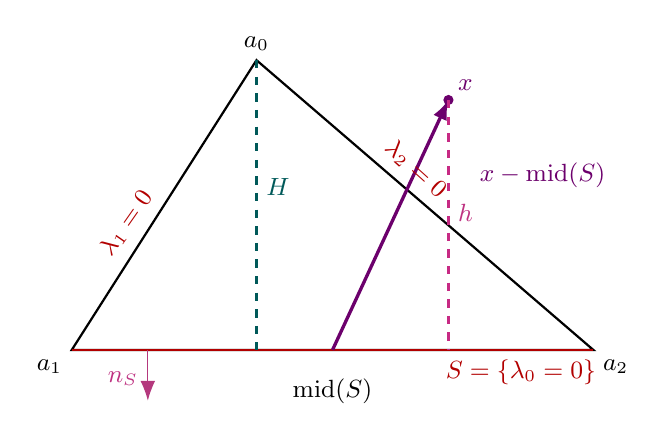
\begin{tikzpicture}[scale=0.92,>=Latex,
    every node/.style={font=\small}]
    \coordinate (a1) at (0,0);
    \coordinate (a2) at (7.2,0);
    \coordinate (a0) at (2.55,4.0);
    \coordinate (m) at (3.6,0);
    \coordinate (foot) at (2.55,0);
    \coordinate (x) at (5.20,3.45);
    \coordinate (xp) at (5.20,0);
    \draw[thick] (a1)--(a0)--(a2)--cycle;
    \draw[red!70!black,thick] (a1)--(a2);
    \draw[teal!70!black,dashed,thick] (a0)--(foot);
    \node[teal!70!black,right] at (2.55,2.25) {$H$};
    \node[below left] at (a1) {$a_1$};
    \node[below right] at (a2) {$a_2$};
    \node[above] at (a0) {$a_0$};
    \node[below=7pt] at (m) {$\midS$};
    \node[red!70!black,below] at (6.20,0) {$S=\{\lambda_0=0\}$};
    \draw[violet!85!black,very thick,-{Latex[length=2.5mm]}] (m)--(x);
    \fill[violet!85!black] (x) circle (2pt);
    \node[violet!85!black,above right] at (x) {$x$};
    \node[violet!85!black,above] at (6.5,2.1) {$x-\midS$};
    \draw[magenta!80!black,dashed,thick] (x)--(xp);
    \node[magenta!75!black,right] at ($(xp)!0.55!(x)$) {$h$};
    \node[red!70!black,rotate=55] at (0.75,1.75) {$\lambda_1=0$};
    \node[red!70!black,rotate=-42] at (4.75,2.5) {$\lambda_2=0$};
    % \node[red,sloped,above=4pt] at ($(a1)!0.52!(a0)$) {$\lambda_2=0$};
    \draw[magenta!70!black,-{Latex[length=2.5mm]}] (1.05,0)--(1.05,-0.7);
    \node[magenta!75!black,left] at (1.05,-0.40) {$n_S$};
\end{tikzpicture}
\caption{Triangle $T$ with facet $S=\{\lambda_0=0\}$, midpoint $\operatorname{mid}(S)$, outward normal $n_S$, altitude $H$, and distance $h$ from $x$ to $S$.}
\end{figure}



Let $h$ be the perpendicular distance from $S$ to $x$, and $H$ be the altitude of the triangle above $S$.

\begin{enumerate}[label=\roman*)]
    \item For any $x \in \mathbb{R}^2,$ can write
    \begin{equation}
        x=\lambda_0(x)a_0+\lambda_1(x)a_1+\lambda_2(x)a_2.
    \end{equation}

    \item Take any $p\in S$. Then
    \begin{align}
        x-p
         &=\lambda_0a_0+\lambda_1a_1+\lambda_2a_2-p\\
         &=\lambda_0a_0+\lambda_1a_1+\lambda_2a_2
            -(\lambda_0+\lambda_1+\lambda_2)p\\
         &=\lambda_0(a_0-p)+\lambda_1(a_1-p)
               +\lambda_2(a_2-p).
    \end{align}

    \item Therefore,
    \begin{equation}
    \begin{aligned}
        n_S\cdot(x-p)
          ={}&\lambda_0n_S\cdot(a_0-p)\\
             &+\lambda_1n_S\cdot(a_1-p)\\
             &+\lambda_2n_S\cdot(a_2-p).
    \end{aligned}
    \end{equation}

    \item Since $a_1-p$ and $a_2-p$ lie along $S$,
    \begin{equation}
        n_S\cdot(x-p)=\lambda_0n_S\cdot(a_0-p).
    \end{equation}

    \item Since $n_S$ is the outward normal, $n_S\cdot(a_0-p)$ projects $a_0-p$ onto the $n_S$ direction.

    \begin{figure}[htbp]
    \centering
    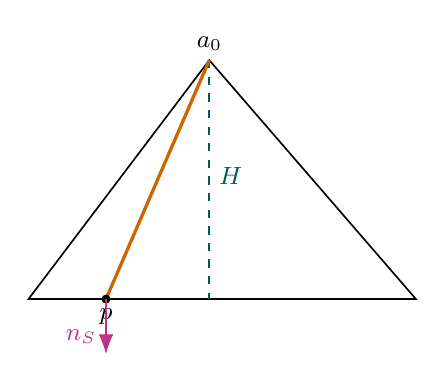
\begin{tikzpicture}[scale=0.82,>=Latex,every node/.style={font=\small}]
       \coordinate (A) at (0,0);
       \coordinate (B) at (6,0);
       \coordinate (C) at (2.8,3.7);
       \coordinate (p) at (1.2,0);
       \coordinate (h) at (2.8,0);
       \draw[semithick] (A)--(B)--(C)--cycle;
       \draw[teal!70!black,dashed,thick] (C)--(h);
       \draw[orange!80!black,very thick] (p)--(C);
       \fill (p) circle (2pt);
       \node[below] at (p) {$p$};
       \node[above] at (C) {$a_0$};
       \node[teal!70!black,right] at (2.8,1.9) {$H$};
       \draw[magenta!75!black,-{Latex[length=2.5mm]}] (p)--++(0,-0.85);
       \node[magenta!75!black,left] at ($(p)+(0,-0.58)$) {$n_S$};
    \end{tikzpicture}
    \end{figure}

    Thus,
    \begin{align}
        n_S\cdot(a_0-p)&=-H,\\
        \Longrightarrow\qquad n_S\cdot(x-p)&=-\lambda_0H,\\
        \Longrightarrow\qquad \lambda_0&=-\frac{n_S\cdot(x-p)}{H},\\
        \Longrightarrow\qquad \lambda_0&=-\frac{n_S\cdot(x-\midS)}{H}.
    \end{align}

    \item With this,
    \begin{equation}
        \text{Carstensen's } \chi_s
          =n_S\cdot(x-\midS)=-H_S\lambda_0.
    \end{equation}

    \item Thus, up to a constant multiple, our choice
    \begin{equation}
        v=-C\lambda_0(\lambda_1\lambda_2)^2\phi_i
    \end{equation}
    is equivalent to Carstensen's
    \begin{equation}
        v=C(\lambda_1\lambda_2)^2
                  \bigl(n_S\cdot(x-\midS)\bigr)\phi_i.
    \end{equation}
\end{enumerate}


\newpage

% --------------------------------------------------------------------
% Handwritten source: pages 11--12
% --------------------------------------------------------------------
\section{Proposed Implementation}

With this equivalence, our implementation can easily be built upon Pablo's.

\subsection{First local problem}
Take
\begin{equation}
    v_1=(\bubbles)^2v,
    \qquad v\in\mathrm{DG}_r,
\end{equation}
and solve
\begin{equation}
    (R_T,v_1)_T=r_T(v_1).
\end{equation}

\subsection{Second local problem}
We have $\qtest$, which is a broken $\mathrm{FB}_{\dim+r}$ space. On $S$,
$q\in\qtest$ has trace $q|_S=\lambda_1\lambda_2p$ for
$p\in\PP_r(S)$.

Thus, we multiply $q\in\qtest$ by $-\bubbles$ and take
\begin{align}
    v_2&=-\bubbles\,q,\\
    v_2|_S&=0,\\
    \left.\partial_{n_S}v_2\right|_S
       &= - C \tilde C(\lambda_1\lambda_2)^2p,
              \qquad p\in\PP_r(S),
\end{align}
% as desired, up to a nonzero normalisation constant.

\subsection{Third local problem}
Now we want $v=(\lambda_1\lambda_2)^2\phi_i$ on $S$.
Thus, take
\begin{equation}
    v_3=\cones\,v,
    \qquad v\in\qtest.
\end{equation}
Then
\begin{equation}
    v_3|_S=(\lambda_1\lambda_2)^2p,
        \qquad p\in\PP_r(S).
\end{equation}

\newpage
% --------------------------------------------------------------------
% Handwritten source: pages 13--16
% --------------------------------------------------------------------
\section{Issues and Questions}
\subsection{Issue 1: Propagation of errors}

\subsubsection*{First local problem}
Take
\begin{equation}
    v_1=b_T^2p,\qquad p\in\PP_r(K),
\end{equation}
and solve
\begin{equation}
    r_T(v_1)=(R_T,v_1)_T.
\end{equation}

The error satisfies
\begin{equation}
    (R_T-R_T^h,b_T^2p)_K=0,
       \qquad \forall\,p\in\PP_r(K).
\end{equation}

If $R_T\in\PP_r(K)$, then we must have
\begin{equation}
    R_T=R_T^h\qquad\text{(Galerkin orthogonality)}.
\end{equation}
If not, we at most get the $b_T^2$-weighted $L^2$-projection of $R_T$ onto $\PP_r(T)$ and we can at most say that
\begin{equation}
    (R_T-R_T^h,b_T^2p)=0,
       \qquad \forall\,p\in\PP_r(T).
\end{equation}

\subsubsection*{Second local problem}
The exact $\Rone$ solves
\begin{equation}
    r_T(v_2)=(R_T,v_2)_T+(\Rone,\dn v_2)_S,
\end{equation}
where $v_2=-\bubbles\,\qtest$.

When we solve the problem in a finite-dimensional space, we satisfy
\begin{align}
    (\Roneh,\dn v_2)_S
       &=r_T(v_2)-(R_T^h,v_2)_T\\
       &=(R_T,v_2)_K+(\Rone,\dn v_2)_S
                                -(R_T^h,v_2)_T.
\end{align}
Consequently,
\begin{equation}
    (\Roneh-\Rone,\dn v_2)_S
      =(R_T-R_T^h,v_2)_T.
\end{equation}

If we recovered $R_T$ exactly, then
\begin{equation}
    (\Roneh-\Rone,\dn v_2)_S=0,
\end{equation}
so $\Roneh$ is the $(\beta_S^T)^2$-weighted projection of $\Rone$.

If, in addition, $\Rone\in\PP_r(S)$, then
\begin{equation}
    \Roneh=\Rone.
\end{equation}

If neither $R_T=R_T^h$ nor $\Roneh=\Rone$, we are stuck with
\begin{equation}
    (\Roneh-\Rone,\dn v_2)_S
      =(R_T-R_T^h,v_2)_T.
\end{equation}

\subsubsection*{Third local problem}
The same idea applies. Take
\begin{equation}
    v_3=\cones\,\qtest.
\end{equation}
Then
\begin{equation}
    r_T(v_3)
      =(R_T,v_3)_T+(\Rzero,v_3)_S
       +\sum_{F\subset\partial T}(\Rone|_F,\dn v_3)_F.
\end{equation}

We solve
\begin{align}
    (\Rzeroh,v_3)_S
      ={}&r_T(v_3)-(R_T^h,v_3)_T\\
         &-\sum_F(\Roneh|_F,\dn v_3)_F\\
      ={}&(R_T,v_3)_T+(\Rzero,v_3)_S\\
         &+\sum_F(\Rone|_F,\dn v_3)_F\\
         &-(R_T^h,v_3)_T\\
         &-\sum_F(\Roneh|_F,\dn v_3)_F.
\end{align}

Thus,
\begin{align}
    (\Rzeroh-\Rzero,v_3)_S
       ={}&(R_T-R_T^h,v_3)_T\\
          &+\sum_F(\Rone-\Roneh,\dn v_3)_F.
\end{align}

And the same analysis applies:
\begin{equation}
    R_T=R_T^h,
    \qquad \Rone=\Roneh
    \quad\Longrightarrow\quad
    \text{we get the $(\beta_S^T)^2$-weighted projection of $\Rzero$.}
\end{equation}
Otherwise, we are stuck with error propagation.

\subsection{Issue 2: What do these test functions look like on $T$?}

\begin{itemize}
    \item Ideally, we want test functions similar to Rognes and Logg.
    \item Using $\qtest$, we get the right structure on $S$, but what do we get on all of $T$? How does that affect our results?
\end{itemize}

\subsection{Question 1: Comparing Pablo's Implementation to Rognes and Logg}

 How does $\qtest$ compare to the $\beta_S^T\phi_i$ used by Rognes and Logg? Rognes and Logg enforce $\beta_S^T \phi_i$ on the whole cell. Pablo uses $\qtest$ which is equivalent to Rognes and Logg's test function on the facet $S,$ but differs on thw whole cell. What impact does that difference have? 


\subsection{Question 2: Does this hold on a general simplex?}

Rognes and Logg's work holds for a general simplex. Carstensen's cone is used under the assumption that the cells of the mesh are triangles. Thus, we implicitly assume that here. However, I wonder if our cones/bubbles apply to the more general case? I think so, but I have to confirm!


\end{document}